\section{Квантовые числа электрона. Принципы заполнения орбиталей. Электронная формула атома и иона. Диаграмма энергетических уровней атома.}

\subsection{Квантовые числа}
Состояние электрона в атоме описывают с помощью четырех квантовых чисел: главного (n), орбитального (l), магнитного (m) и спинового (s).

 

\Def{Главное квантовое число}

Определяет энергетический уровень электрона, принимает целые значения $(n = 1, 2, 3 ...)$. Номер периода атома = число энергетических уровней атома.

Например:

Элемент кадмий Cd расположен в пятом периоде, значит $n = 5$. В его атоме электроны раcпределены по пяти энергетическим уровням $(n = 1, n = 2, n = 3, n = 4, n = 5)$; внешним будет пятый уровень $(n = 5)$. 

\Def{Орбитальное квантовое число}

 Характеризует геометрическую форму орбитали. Принимает значение целых чисел от 0 до (n - 1). Набор орбиталей с одинаковыми значениями n называется энергетическим уровнем, c одинаковыми n и l - подуровнем. Обозначаются буквами s,p,d,f...
 
 \Def{Магнитное квантовое число} 
 
 Принимает целочисленные значения от -l до +l. 
 
 \subsection{Принципы заполнения орбиталей}
 
\Def{Принцип Паули}
 
 В атоме может быть двух электронов, у которых значения всех квантовых чисел (n, l, m, s) были бы одинаковы, т.е. на каждой орбитали может находиться не более двух электронов (c противоположными спинами).
 
 \Def{Правило Клечковского (принцип наименьшей энергии)}:
 
 Заполнение электронами орбиталей в атоме происходит в порядке возрастания суммы главного и орбитального квантовых чисел n + l. При одинаковой сумме раньше заполняется орбиталь с меньшим значением n.

1s < 2s < 2p < 3s < 3p < 4s < 3d < 4p < 5s < 4d < 5p < 6s < 5d < 4f < 6p < 7s

 \Def{Правила Хунда}
 
 \begin{itemize}
     \item Минимальной энергией обладает терм с максимальным значением S
     \item Из термов с одинаковым значением S наименьшей энергией обладает терм с максимальным значением L
 \end{itemize}
 
 \subsection{Электронная формула атома и иона}
 
 Максимальное число электронов на энергетическом уровне равно $2n^2$ (n - номер энергетического уровня).
 
 Энергетический уровень может быть завершенным или незавершенным. В завершенном энергетическом уровне все орбитали заполнены, электроны спарены.

Заполнение энергетических уровней идет по принципу наименьшей энергии. Электрон занимает орбиталь с наименьшей энергией.

\begin{figure}[H]
    \centering
    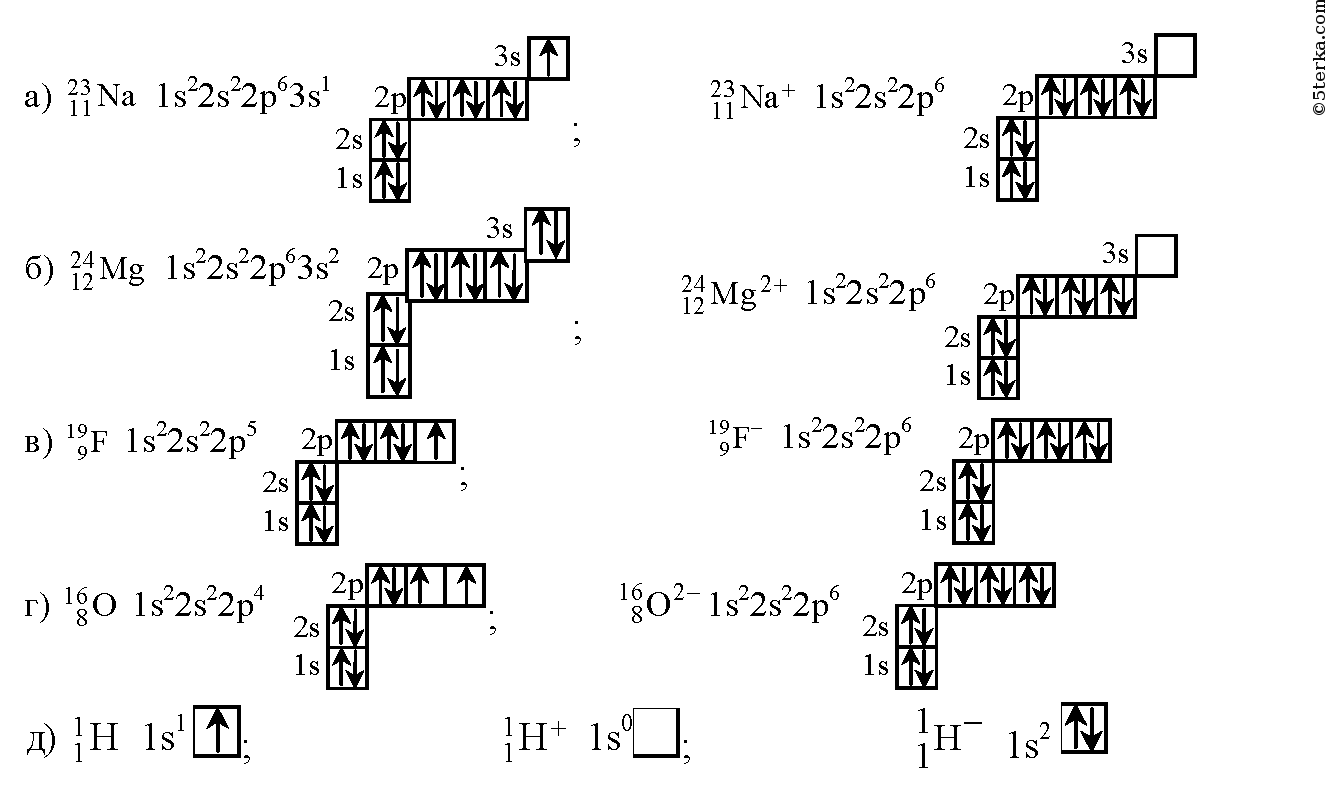
\includegraphics[width = \textwidth]{Pictures/6_atom.png}
    \caption{Примеры формул электронного строения и диаграмм уровней}
    \label{fig:7atom}
\end{figure}

